\section{Perkalian}
\subsection{Pengertian dasar perkalian biner}
Perkalian dalam biner mirip dengan pasangan desimalnya. Dua angka A dan B dapat dikalikan dengan produk parsial: 
untuk setiap digit di B, produk dari digit di A dihitung dan ditulis pada baris baru, bergeser ke kiri sehingga 
garis digit paling kanannya naik dengan angka di B yang bekas. Jumlah semua produk parsial ini memberikan hasil akhir.

\subsection{definisi hexadesimal}
Sistem angka heksadesimal, yang juga dikenal sebagai hex, adalah sistem angka yang terdiri dari 16 simbol (dasar 16). 
Sistem angka standar disebut desimal (basis 10) dan menggunakan sepuluh simbol: 0,1,2,3,4,5,6,7,8,9. Heksadesimal 
menggunakan angka desimal dan mencakup enam simbol tambahan. Tidak ada simbol yang berarti sepuluh, atau sebelas, 
jadi simbol ini diambil dari alfabet Inggris: A, B, C, D, E dan F. Heksadesimal A = desimal 10, dan heksadesimal F = desimal 15

Manusia kebanyakan menggunakan sistem desimal. Ini mungkin karena manusia memiliki sepuluh jari (sepuluh digit). 
Komputer bagaimanapun, hanya memiliki on dan off, disebut digit biner (atau sedikit, singkatnya). Nomor biner 
hanyalah string angka nol dan angka: 11011011, misalnya. Untuk kenyamanan, insinyur yang bekerja dengan komputer 
cenderung mengelompokkan bit bersama-sama. Pada hari-hari sebelumnya, seperti tahun 1960-an, mereka akan mengelompokkan 
3 bit sekaligus (seperti bilangan desimal besar dikelompokkan dalam tiga tingkat, seperti angka 123.456.789). Tiga bit, 
masing-masing dinyalakan atau dimatikan, dapat mewakili delapan bilangan dari 0 sampai 7: 000 = 0; 001 = 1; 010 = 2;
011 = 3; 100 = 4; 101 = 5; 110 = 6 dan 111 = 7. Ini disebut oktal

\subsection{sistem bilangan hexadesimal terhadap desimal}
Heksadesimal atau sistem bilangan basis 16 adalah sebuah sistem bilangan yang menggunakan 16 simbol. Berbeda dengan sistem bilangan desimal, 
lambang yang dipakai dari sistem ini yaitu angka 0 sampai 9, ditambah dengan 6 lambang lainnya menggunakan huruf A sampai F. Sistem 
bilangan ini digunakan untuk menampilkan nilai alamat memori dalam pemrograman komputer.

\subsection{Pengertian luas hexadesimal}
Dalam matematika dan komputasi, heksadesimal (juga basis 16, atau heks) adalah sistem angka posisional dengan radix, atau basis, dari 16. Ini 
menggunakan enam belas simbol yang berbeda, paling sering simbol 0-9 untuk mewakili nilai nol sampai sembilan, dan A, B, C, D, E, F (atau 
alternatif a, b, c, d, e, f) untuk mewakili nilai sepuluh sampai lima belas. Angka heksadesimal banyak digunakan oleh perancang dan pemrogram 
sistem komputer. Karena setiap digit heksadesimal mewakili empat digit biner (bit), ini memungkinkan representasi biner yang lebih ramah manusia. 
Satu digit heksadesimal mewakili nibble (4 bit), yang merupakan setengah dari oktet atau byte (8 bit). Sebagai contoh, satu byte dapat memiliki 
nilai mulai dari 00000000 sampai 11111111 dalam bentuk biner, tapi ini mungkin lebih mudah direpresentasikan sebagai 00 sampai FF dalam heksadesimal.
Dalam konteks non-pemrograman, subskrip biasanya digunakan untuk memberi radix, misalnya nilai desimal 10.995 akan dinyatakan dalam heksadesimal 
sebagai 2AF316. Beberapa notasi digunakan untuk mendukung representasi heksadesimal dari konstanta dalam bahasa pemrograman, biasanya melibatkan 
awalan atau akhiran. Awalan 0x digunakan dalam bahasa C dan bahasa terkait, di mana nilai ini dapat dinotasikan sebagai 0x2AF3.

\subsection{contoh perkalian biner}

\subsubsection{Perkalian dengan 3}
Dari Tabel 1 dapat ditentukan
Satuan Hasil Perkalian dengan 3 (SHP3)
k 0 2 4 6 8
SHP3 0 6 2 8 4
Jika k genap maka:
SHP3 = Nilai satuan pada : 2 (10 - k)
k 1 3 5 7 9
SHP3 3 9 5 1 7
Jika k ganjil maka:
SHP3 = Nilai satuan pada : 2 (10 - k) + 5
Sehingga cara mudah menentukan hasil
perkalian bilangan n digit dengan 3 :
1. Untuk angka terkanan =
Nilai satuan pada : 2 (10- k), k genap
Nilai satuan pada : 2 (10- k) + 5,
k ganjil
Jika memuat puluhan simpan sebagai
simpanan
2. Untuk angka di sebelah kirinya =
Nilai satuan pada : 2 (9- k), k genap
Nilai satuan pada : 2 (9- k) + 5,
k ganjil, ditambah s dari
Jurnal Matematika Vol. 11, No.1, April 2008:38-42
40
tetangganya.
Jika dari langkah 1 diperoleh
simpanan maka simpana yang ada
ditambahkan pula.
Jika hasilnya memuat puluhan simpan
sebagai simpanan
3. Ulangi langkah 2 sampai digit ke n
4. Untuk digit ke (n+1) =
s dari digit ke n + ”simpanan”
dikurangi 2
Dengan demikian jika bilangan yang
dikalikan n digit diperlukan (n+1) langkah
Contoh:
( 1 ) 9876 X 3 = ?
Penyelesaian : Pandang 09876
Langkah 1 : 2 (10-6) = 2 (4) = 8
Langkah 2 : 2 (9-7)+5+”s” dari 6
= 2 (2)+5+3=4+5+3 = 12
= 2 simpan 1
Langkah 3 : 2 (9-8)+
”s” dari 7 + simpanan
= 2(1)+3+1=2+3+1= 6
Langkah 4 : 2 (9-9)+5+”s” dari 8
= 2 (0)+5+4=0+5+4 = 9
Langkah 5 : s dari 9 – 2 = 4-2 = 2
Maka : 9876 X 3 = 29628.
Atau dikerjakan dengan cara lain :
( 2 ) 41692573 X 3 = ?
C = simpanan, H = hasil
k OPERASI C H
3 2(10-3)+5 = 19 1 9
7 2(9-7)+5+1+1 1 1
5 2(9-5)+5+3+1 1 7
2 2(9-2)+2+1 1 7
9 2(9-9)+5+1+1 0 7
6 2(9-6)+4+0 1 0
1 2(9-1)+5+3+1 2 5
4 2(9-4)+0+2 1 2
0 2+1-2 0 1
Jadi 41692573 X 3 = 125077719

\begin{figure}[ht]
	\centerline{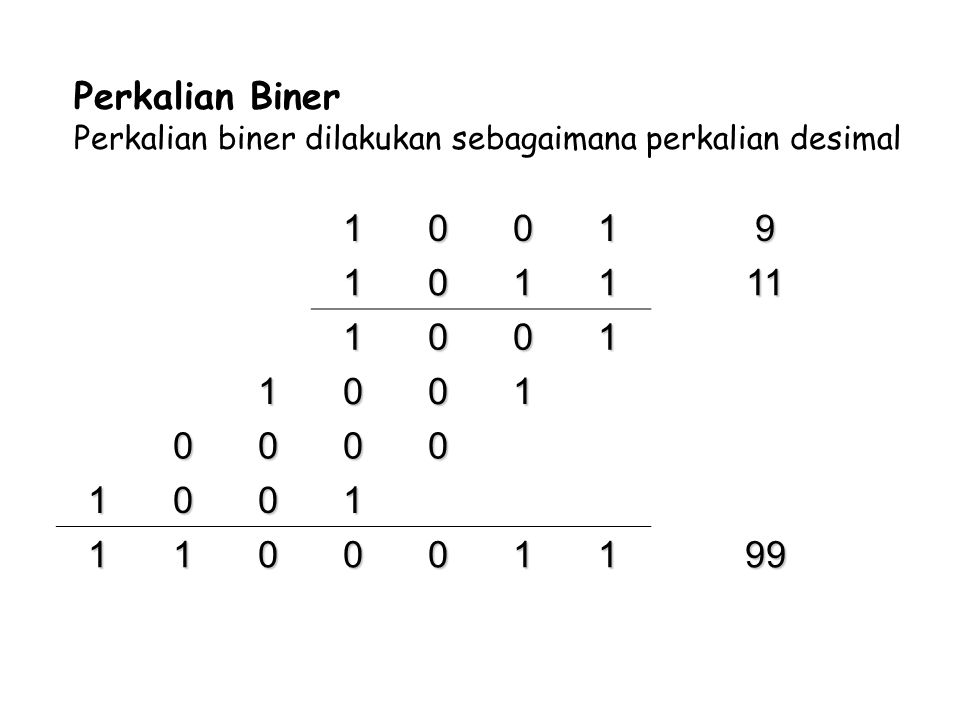
\includegraphics[width=1\textwidth]{figures/perkalianbiner.jpg}}
	\caption{gambar dari perkalian biner.}
	\label{perkalian}
\end{figure}
\subsubsection{Perkalian dengan 4}
Dari Tabel 1 dapat ditentukan
Satuan Hasil Perkalian dengan 4 (SHP4)
k 0 2 4 6 8
SHP4 0 8 6 4 2
Jika k genap maka :
SHP4 = 10- k
k 1 3 5 7 9
SHP4 4 2 0 8 6
Jika k ganjil maka:
SHP4 = 15- k
Sehingga cara mudah menentukan hasil
perkalian bilangan n digit dengan 4 :
1. Untuk angka terkanan =
Nilai satuan di : 10 - k, k = genap
Nilai satuan di : 15 - k, k = ganjil
Jika memuat puluhan simpan sebagai
simpanan
2. Untuk angka di sebelah kirinya =
Nilai satuan pada : (9- k)+ s dari
tetangganya, k genap
Nilai satuan pada : (9- k) + s dari
tetangganya + 5, k ganjil
Jika dari langkah 1 diperoleh
simpanan maka simpana yang ada
ditambahkan pula.
Jika hasilnya memuat puluhan simpan
sebagai simpanan
3. Ulangi langkah 2 sampai digit ke n
4. Untuk digit ke (n+1) =
 s dari digit ke n + ”simpanan”-1
Contoh :
( 1 ) 4765 X 4 = ?
Penyelesaian :
C = simpanan , H = hasil
k OPERASI C H
5 15-5 1 0
6 (9-6)+2+1 0 6
7 (9-7)+3+5+0 1 0
4 (9-4)+3+1 0 9
0 2-1+0 0 1
Jadi 4765 X 4 = 19060
( 2 ) 87645912 X 4 = ?
Penyelesaian :
C = simpanan , H = hasil
k OPERASI C H
2 10-2 0 8
1 (9-1)+1+5+0 1 4
9 (9-9)+0+5+1 0 6
5 (9-5)+4+5+0 1 3
4 (9-4)+2+1 0 8
6 (9-6)+2+0 0 5
7 (9-7)+3+5+0 1 0
8 (9-8)+3+1 0 6
0 4-1+0 0 3
Jadi 87645912 X 4 = 360583648
Putut Sriwasito (Perkalian Biner Bilangan N Digit Dengan 3, 4, 5 dan 6)
41

\subsection{Pengenalan Warna Citra Binary}
Citra biner (binary image) adalah citra yang hanya mempunyai dua nilai derajat: Meskipun saat ini citra berwarna lebih disukai karena memberi kesan yang lebih 
kaya dari pada citra biner, namun tidak membuat citra biner mati. Pada beberapa aplikasi citra biner masih tetap dibutuhkan, misalnya citra logo instansi (yang
hanya terdiri atas warna hitam dan putih), citra kode batang (bar code) yang tertera pada label barang, citra hasil pemindahan dokumen teks, dan sebagainya.
objek di dalam citra biner adalah segmentasi objek. Proses segmentasi  mempunyai tujuan untuk menyatukan pixel-pixel obyek menjadi daerah (region) yang merepresentasikan 
obyek. Ada dua pendekatan yang digunakan dalam segmentasi objek:


	
	
\subsubsection{Perkalian dengan 6 Perkalian dengan 5}
Dari Tabel 1 dapat ditentukan
Satuan Hasil Perkalian dengan 5 (SHP5)
k 0 2 4 6 8
SHP5 0 0 0 0 0
Jika k genap maka :
SHP5 = 0
k 1 3 5 7 9
SHP5 5 5 5 5 5
Jika k ganjil maka:
SHP5 = 5
Sehingga cara mudah menentukan hasil
perkalian bilangan n digit dengan 5 :
1. Untuk angka terkanan = 0, k genap
5, k ganjil
2. Untuk angka di sebelah kirinya =
0+ s dari tetangganya, k genap
5+ s dari tetangganya + 5, k ganjil
3. Ulangi langkah 2 sampai selesai
Contoh:
( 1 ) 7896 X 5 = ?
Penyelesaian:
H = hasil
k OPERASI H
6 0
9 5+3 8
8 0+4 4
7 5+4 9
0 0+3 3
Jadi 7896 X 5 = 39480
( 2 ) 86532947 X 5 = ?
Penyelesaian:
H = hasil
k OPERASI H
7 5
4 0+3 3
9 5+2 7
2 0+4 4
3 5+1 6
5 5+1 6
6 0+2 2
8 0+3 3
0 0+4 4
Jadi 865

\subsection{Hexa 3}
Seiring komputer bertambah besar, lebih mudah mengelompokkan bit menjadi empat, bukan tiga. Ini menggandakan 
angka yang akan ditunjukkan simbol; itu bisa memiliki 16 nilai bukan delapan. Hex = 6 dan Desimal = 10, sehingga 
disebut heksadesimal. Empat bit disebut menggigit (kadang dieja nybble). Menggigit adalah satu digit heksadesimal, 
dan ditulis menggunakan simbol 0-9 atau A-F. Dua camilan adalah byte (8 bit). Sebagian besar operasi komputer 
menggunakan byte, atau kelipatan byte (16 bit, 24, 32, 64, dll.). Heksadesimal memudahkan penulisan bilangan biner besar ini.


\subsection{contoh perkalian}
10111 by 1101

Solution:

                                1 0 1 1 1

                                   1 1 0 1

                                 1 0 1 1 1           ← First partial product

                            1 0 1 1 1     

                            1 1 1 0 0 1 1           ← First intermediate sum

                         1 0 1 1 1          

                       1 0 0 1 0 1 0 1 1           ← Final sum.

Hence the required product is 100101011.


(ii) 11011.101 by 101.111

                                        1 1 0 1 1 . 1 0 1

                                             1 0 1 . 1 1 1  

                                        1 1 0 1 1 . 1 0 1

                                     1 1 0 1 1 1 . 0 1          ← First partial product

                                  1 0 1 0 0 1 0   1 1 1        ← First intermediate sum

                                  1 1 0 1 1 1 0   1        

                               1 1 0 0 0 0 0 1   0 1 1    ← Second intermediate sum

                               1 1 0 1 1 1 0 1              

                             1 1 0 0 1 1 1 1 0   0 1 1        ← Third intermediate sum

                          1 1 0 1 1 1 0 1                    

                       1 0 1 0 0 0 1 0 0 1 0   0 1 1
		     
\subsection{Perkalian Dua-komplemen}
•
Urutan penambahan pelengkap ganda dari multiplicands bergeser
kecuali untuk langkah terakhir dimana multiplicand bergeser sesuai dengan MSB
harus ditiadakan
•
Sebelum menambahkan multiplicand bergeser ke produk parsial, tambahan
bit ditambahkan ke kiri dari produk parsial menggunakan tanda ekstensi.
Ex:
- 5 1011 multiplicand
x
- 3 x
 Pengganda 1101
 15 00000 produk parsial
                                            11011 bergeser multiplikand
                                          111011 produk parsial
                                         00000 bergeser multiplicand
                                       1111011 produk parsial
                                       11011 bergeser multiplikand
                                     11100111 produk parsial
                                     00101 bergeser dan meniadakan perkalian
                                     Produk 00001111
									 

\subsection{Perkalian Decimal}
Untuk mengalikan dua angka desimal berganda, pertama Anda harus tahu bagaimana mengalikan dua angka desimal satu digit. Ini memerlukan penghafalan 100 fakta, 
atau 55 fakta jika Anda mengecualikan fakta komutatif atau perputaran. Fakta ini biasanya diwakili dalam tabel perkalian, juga dikenal sebagai tabel 
waktu. 
Contoh fakta adalah 2 x 9 = 18, 9 x 7 = 63, dan 1 x 6 = 6.


\subsection{mengubah bilangan hexadesimal ke biner}

dalam sebuah artikel oleh Jeperson Hutahaean yang menyatakan bahwa contoh bilangan hexadesimal adalah 5D9316, dan cara konversi ke bilangan biner adalah 
sebagai berikut:
hexa  ->  biner
5     ->  0101
D     ->  1101
9     ->  1001
3     ->  0011

 catatan : 

- jadi bilangan benir untuk heks 5D9316 adalah 0101110110010011.
- untuk lebih jelasnya dapat dilihat tabel Digit Heksadesimal di bawah.

\cite{smith1999mode}
\cite{schwarz1997implementation}
\cite{nurhayati2010aritmatik}
\cite{sriwasito2010perkalian}